\chapter{Initial Analysis}\label{chap:analysis}
The following analysis will investigate the initial knowledge to form the design requirements and a final problem statement for the report. The analysis is based on a case taken from the company Zoo, explained in the introduction of the report.



\section{Problem area}\label{problemArea}
As mentioned in \autoref{intro}, Copenhagen Zoo introduced potential problems that could be solved. In order to establish a clear understanding of the defined problems, aswell as other general issues, a meeting with Christian Astorp from Copenhagen Zoo was held.

The meeting with Christian Astorp \todo{Få bekræftet at vi må nævne ham med navn i rapporten} elaborated on limitations, needs and wishes, and provided an opportunity to exchange ideas for possible solutions. During the meeting, it became clear that an important aspect of the project, would be to maintain the spirit of Zoo, by staying true to the nature of the animals, and creating a family friendly, informative, experience based around the animals. The meeting also provided a potential target group as well as general requirements for the project.
The following is a descriptive guideline for the project, based on the needs and wishes of Zoo:   \\

\begin{itemize}
    \item[-] The solution should be implemented as a hands-free digital display. The park has several installations with physical buttons, but these solutions has high maintenance, as children aren't considerate enough when using them. 
    \item[-] The installation should add value to the user, in terms of an experience they otherwise wouldn't have had in the park. 
    \item[-] The experience must concern the animals located in same area as the installation, to achieve a coherent experience.
    \item [-] The experience should be informative\todo{Not a direct necessary requirement}.
    \item[-] If animals are to be represented, it must be done in respect to the natural behavior of the animal. An example of a violation of this would be to humanize the animals by, for instance, animating talking animals. 
    \item[-] The experience should not be age specific, but should preferably primarily appeal to children, and secondarily their parents, as this target group is the most represented audience in the park. 
    \item[-] The interaction level should be simple and straightforward, and shouldn't need more than the users themselves to be able to perform the interactions. 
    \item[-] The experience should not be dependent on the season, but instead encourage all-year-use. As so, it was suggested to make an experience that could be used in weather conditions where most animals will not be outdoors for the guest to see.
    \item[-] During a guest's visit, the installation should strive to entertain the guests and make them spend time with the installation, such that the entire park is less likely to be explored in one trip. This will make the guest more likely to come back to the park.\todo{Måske skriv om placement af vores solution? Hvilke steder var aktuelle og hvorfor ender vi der hvor vi gør}
    
    
\end{itemize}

    % Baseret på dyr, relevant for omgivelser
    % Saglig, ikke fjollet
    % Informativt
    % Børnehøjde men OGSÅ til voksne!
    % Simple interaktion, ingen controllerer.
   
    % Ikke bundet til en specifik sæson.
    % Gæster skal gå derfra med en oplevelse/ værditilførelse.
    % Design skal gerne kunne holde på folk.

% examples of existing installations in the park.


% possible locations
% statistics about the target group (børn og voksne) 

\subsection{Target Group Analysis}
\todo{Data from Zoo}
After the meeting with Christian Astorp in Zoo, the target group can be defined, as one of the points taken from the meeting was the following:

"The experience should not be age specific, but should preferably primarily appeal to children, and secondarily their parents, as this target group is the most represented audience in the park."

Since a zoo is predominantly a place for families with children (Between 60 to 80\% worldwide)\cite{togetherAtTheZoo} it is relevant to study their shared experience in order to design engaging interactive installations aimed at children without neglecting the parents.
A theoretical framework based on existing literature suggests that \textit{social bonding} with their children is considered the primary experience from the parents' perspective, with \textit{"edutainment"}\footnote{Entertainment that is designed to be educational. Meriam-webster's definition can be seen here: \url{https://www.merriam-webster.com/dictionary/edutainment}} being a secondary goal of a visit at the zoo. Parents are interested in providing learning experiences for their children. However, \textit{entertainment} is the primary goal and \textit{togetherness} the secondary for children\cite{togetherAtTheZoo}. The learning aspect is not a priority for the younger children, at least not during the entire visit. Older children tend to have more curiosity towards detailed knowledge about the animals and read from the information boards together with their parents\cite{togetherAtTheZoo}. Through interviews with families conducted in Aalborg Zoo it was found that, aside from activities involving animals, physical activities in the zoo playground are also central for children when visiting the zoo. The occasional break from passively watching the animals, by partaking in physical activities, helps the children refocus when returning to explore the animals\cite{togetherAtTheZoo}.

Thus, the target group can be defined as the traditional family, primarily children, with the secondary target group be their parents.

\section{Tech Analysis}\label{Tech}
After interviewing Zoo, we have a set of requirements the final product should strive to achieve. The product has to be a digital, interactive installation concerning an animal, that should be placed in the vicinity of that animal in Zoo. As the Zoo requires the product to be used without controllers, an analysis of relevant, hand-free technology will follow.

 \subsection{The Kinect for Xbox One (2013 version)}
        The latest model of the Kinect, uses a time-of-flight camera, along with an infrared camera to track and read the environment\cite{KinectWiki}. The time-of-flight camera measures distance by emitting a pulse of light and then measure the time for the light signal to return in relation to the speed of light. Thereby calculating the distance to each point within the scene.
        
        This Kinect version can track within a 3\todo{WAT?} ft range, detect heart rate and facial expressions of the user, as well as estimate the joints and thereby skeletal composition of up to 6 users at the time\cite{KinectWiki}.
        
        Part owner of an art collective named \textit{Floating Point} Jack Kalish \cite{LANscapes}, used the Kinect in an art installation \textit{LanScape}, where the users/observers movements would manipulate a digital landscape, projected on a wall. The landscape would for example take shape as mountains or valleys if the user would raise their arms or sit on the floor, respectively.
        
        Garratt Gallagher from MIT’s Computer Science and Artificial Intelligence Laboratory (CSAIL) \cite{MR_MIT}, used the Kinect to create an interface similar to the one seen in the fiction film \textit{Minority Report}\footnote{Minority Report: \url{https://en.wikipedia.org/wiki/Minority_Report_(film)}}. The Kinect can as seen, also be used to track gestures and thereby interact with interfaces. 
        
        \subsection{Leap Motion} % Daniel
    Leap motion is a tool that is used for tracking hands and fingers in real time\cite{leapMotion}. The newest iteration integrates with Virtual Reality, hence eliminating the need for having a controller in your hand. The Leap Motion controller functions by having three IR LEDs and two monochromatic IR Cameras. The maximum reading distance from the controller is approximately 1m\cite{leapMotion}. The accuracy of the controller is roughly 0.7mm, hence the virtual version of ones hands can be very precise as seen in \autoref{fig:leapMotion}.
    
    \begin{figure}[H]
    	\centering
    	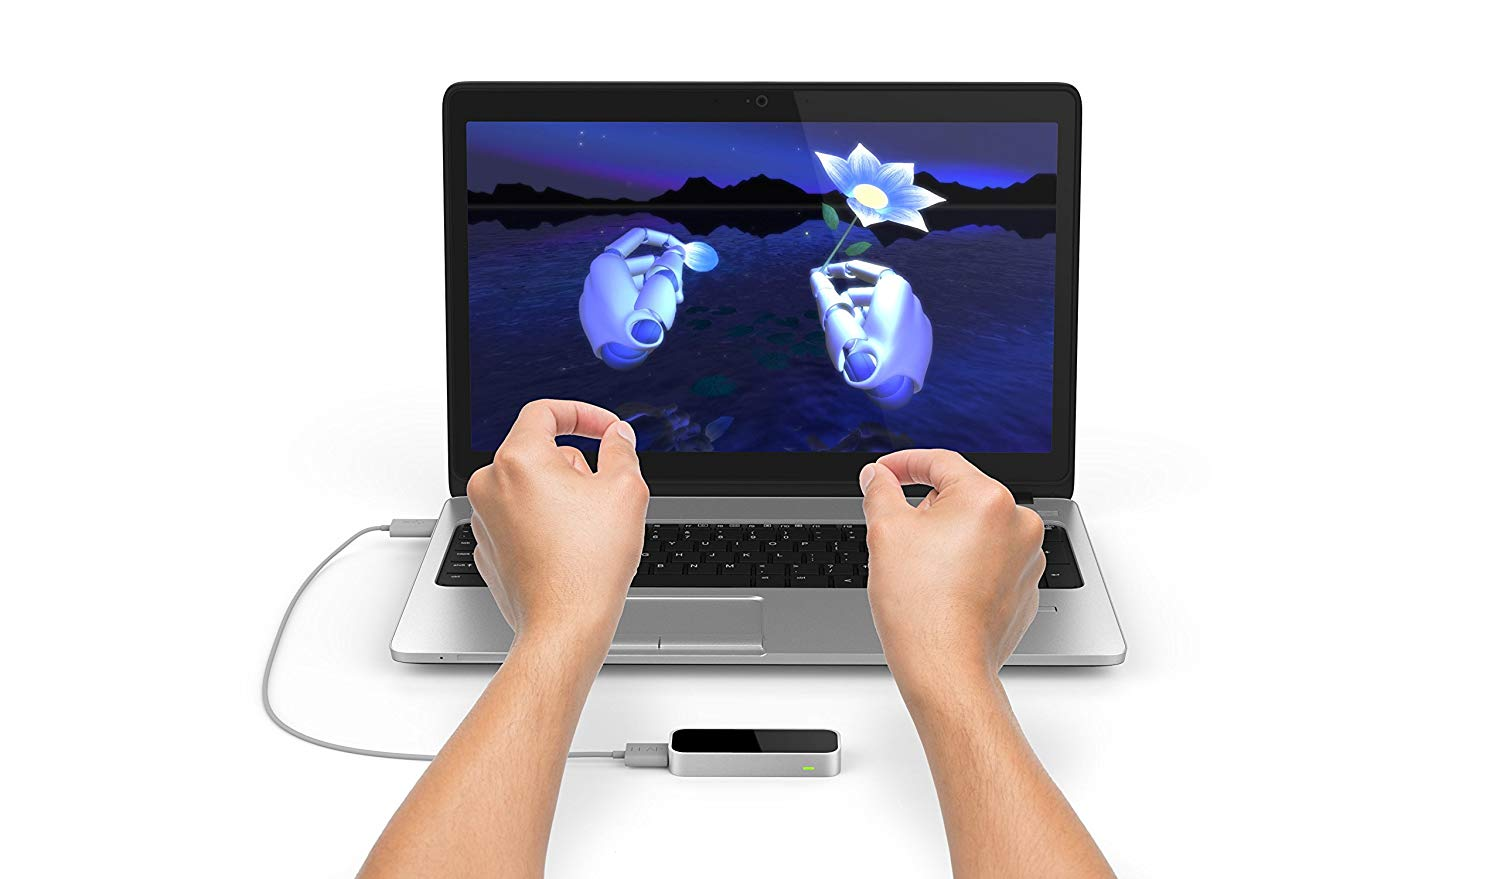
\includegraphics[width=0.9\linewidth]{figure/Analysis/leapMotion.jpg}
    	\caption{Image of the Leap Motion in action, taken from the Amazon store page.}
    	\label{fig:leapMotion}
    \end{figure}
    
    \subsection{Multiple display setups}
As seen in \autoref{sec:leapMotionHolodeck} and \autoref{sec:transcendingBoundaries} multiple projectors working in tandem are utilized to create immersive technology. There are several ways of having multiple projectors working together. Using a Graphical Processing Unit, or GPU for short with sufficient outputs to drive all the required projectors. Newer graphics cards can run up to 4 monitors at the same time \footnote{GTX 1080TI: \url{https://www.evga.com/products/product.aspx?pn=11G-P4-6693-K3}}, or with the use of a display port hub, splitting the bandwidth of the display ports to allow more monitors at lower resolutions\footnote{EVGA DisplayPort Hub\url{https://www.evga.com/products/product.aspx?pn=200-dp-1301-l1}} which makes it possible to run even more screens off a single high end GPU, depending on how many display ports it has. If more monitors than this are needed, multiple GPU's can be installed in the same system, and even more displays can be used. Another way to achieve multiple displays with a single display port is using a technology called daisy chaining. The principle behind this is to connect multiple displays supporting display ports where each one is connected in sequence to each other, hence only requiring one output from the GPU. Depending on the resolution this can be done with 2-5 monitors\cite{displayport}.




\section{Interaction}
This session is investigated in relation to the point found in the problem area: "The interaction level should be simple and straightforward, and should not need more than the users themselves to be able to perform the interactions. Therefore no controllers or wearables must be used".\todo{As Lars mentioned, this paragraph is a bit wonky since we dont have anything to back this claim up with, we need to back it up somehow and then perhaps rephrase}

\subsection{Implicit Human Computer Interaction}
%conc
The point of implicit interactions is that the same subtle principles that governs interactions between people, also controls the interactions with computers\cite{Schmidt2000}.\\
"Sensing and computation need to be augmented with an understanding of the unstated expectations we people have from our interactive counterparts"\cite{Schmidt2000}

By considering how people achieve interaction goals with other people, one could isolate these interactions and apply them to Human Computer Interaction (HCI).

Reeves and Nass coined the Media Equation\cite{mediaequation} which states that interactive objects are engaged with, as if they were real people. This ties together with implicit interaction, as it is based on these interactions. Furthermore, the last of the eight media equation propositions states that people already know how to behave in the real world and therefore this can be translated to computer interaction.

Implicit human computer interaction is important to consider as it differentiates itself from explicit human computer interaction which encompasses more traditional interactions where the user directly expects a reaction from their initial action.

This should be considered when creating a prototype, as the product should include a simple interaction according to the investigation of the problem area in the Zoo. \ref{zoo}

%\section{Perception}
%"Perception is the ability to become aware of something through human senses (hearing, %seeing, feeling etc)\\

% https://ieeexplore.ieee.org/document/1667620/#full-text-section

% https://link.springer.com/article/10.1007/BF00896880

% file:///Users/damh/Downloads/927-3572-1-SM.pdf

% http://diposit.ub.edu/dspace/bitstream/2445/49643/1/631349.pdf

% https://www.interaction-design.org/literature/topics/visual-hierarchy

% https://dzone.com/articles/visual-perception-and-its-influence-in-ux-design-1

\subsection{Interactive public displays} % Daniel
    From an interaction perspective, interactive public displays are different for how the user would usually interact with a display \cite{interactivePublicDisplays}. Mostly this difference comes from the interaction not beginning directly from interacting with the display, but happens in more indirect sense. To better understand why this is, the interaction phases of an interactive public display has been broken down into 6 different stages, as seen in \autoref{fig:audienceFunnel}. A user only goes between phases, when passing a threshold, e.g. for a user to pass into the second phase, their attention must be caught\cite{interactivePublicDisplays}.
    
    \begin{figure}[H]
    	\centering
    	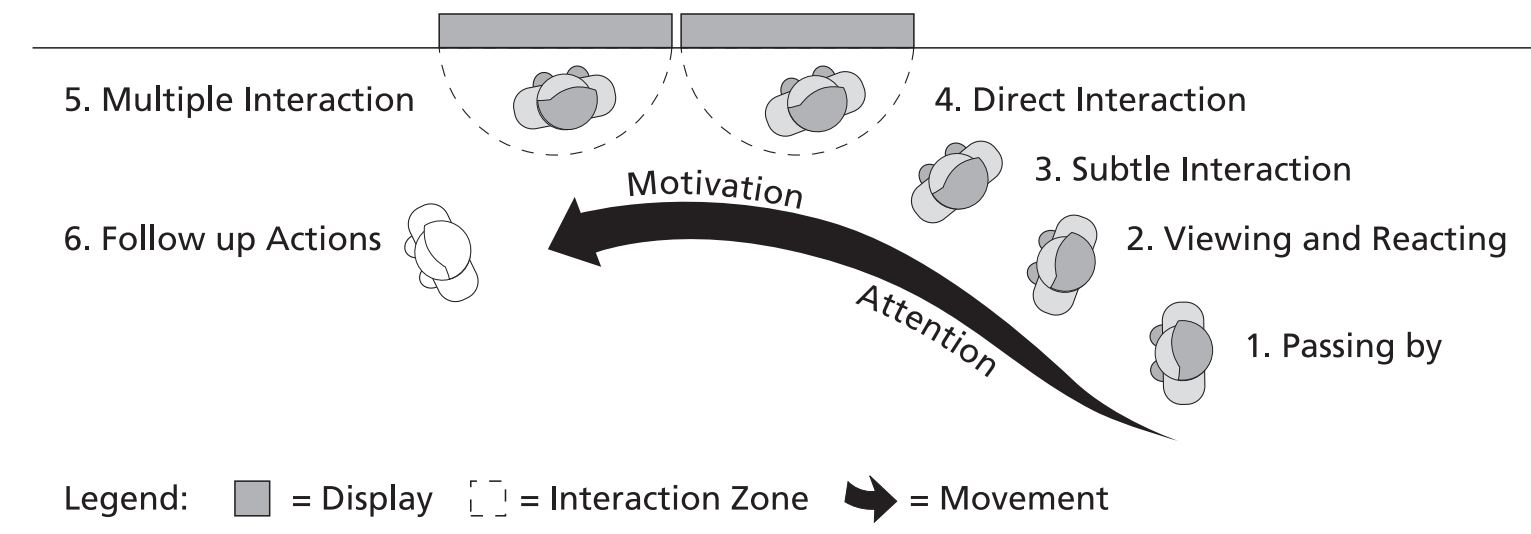
\includegraphics[width=0.9\linewidth]{figure/Analysis/AudienceFunnel.png}
    	\caption{The interaction phases of an interactive public display being broken down into 6 stages, compiled into the audience funnel model\cite{interactivePublicDisplays}.}
    	\label{fig:audienceFunnel}
    \end{figure}
    
    The entire interaction with the display only starts when a potential user's attention gets caught by the display. The attention grabbing mechanism of the display can vary a lot in implementation and style, but can in be broken down into bottom-up processes and top-down processes\cite{interactivePublicDisplays}. Bottom-up processes involve some external stimuli that via something unexpected can help grab attention from a user. This can 
    , for example, >be a suddenly appearing polar bear, an error message, or any other item that the user might not have been looking for\cite{interactivePublicDisplays}. Top-down processes revolve around a user having a form of a goal that will guide their attention towards what they are looking for\cite{interactivePublicDisplays}, e.g. if a user was looking for a penguin, and a penguin was observed in their vision, their attention would be guided towards it.
    
    The second phase is entered after the user has become aware of the existence of the display, and might have turned their head, diverted their gaze towards the display or performed any action affected by the attention to the display\cite{interactivePublicDisplays}.
    
    While in the beginning of the interaction with the display, it is mostly reliant on attention from the user, but when a user is in the third phase, it becomes more dependent on the motivation to interact\cite{interactivePublicDisplays}. This motivation can be increased using curiosity and exploration\cite{interactivePublicDisplays}. Curiosity, according to Müller et al., is described as 
    \begin{quote}
        \textit{"a precursor to explorative behavior, through which people make accessible previously unavailable information about their environment."}\cite{interactivePublicDisplays}
    \end{quote}
    So by presenting some information and leaving out some gaps, or having a puzzle missing one more piece to be finished, the user might become curious and start exploring the possibilities of e.g. putting in the last the piece of the puzzle\cite{interactivePublicDisplays}.
    
    The third phase begins when what was displayed during the second phase, makes the user curious enough to physically divert their body towards the display, or making any movement that is meant to cause the display to react, while not necessarily being in frame of the screen. At this point, it is the goal that the user's motivation to interact is high enough to enter the next phase, direct interaction\cite{interactivePublicDisplays}.
    
    The fourth phase of direct interaction is when a user has either positioned themselves in front of the display, or simply has entered the interaction zone of the display. In the case of the Magical Mirrors mentioned in the article\cite{interactivePublicDisplays}, the interaction zone, was the right dashed circle displayed in \autoref{fig:audienceFunnel}, while the left dashed circle was a secondary screen, that might be used when in phase five; Multiple interaction.
    
    The fifth phase of the interaction is started when a user, in the case of the magical mirrors, either goes from one display to another, or comes back for another interaction after ending the first\cite{interactivePublicDisplays}.
    
    The sixth and final phase the interaction might end with, is the follow up phase, where a user might do an action following up the interaction from the display. This might entail using their smartphone, to search for more information about the display or information gotten from the display during the interaction, or take a photograph of themselves or their friends still doing interaction\cite{interactivePublicDisplays}. 
    
\subsection{The influence of social aspects in public displays} %sofie
The individual possible user's interaction would be established and executed (as described in SECTION XXX), must be considered in relation to how the interaction might be influenced by the presence of multiple bystanders and fellow participants. \\
When designing a public display, one needs to consider how a possible user might become encouraged or discouraged to interact with the display, due to this presence of others. Namely, how to deal with the potential problem social embarrassment, and which elements should be used or avoided, in trying to establish the social affordance called the honey-pot effect. The later, is the term used to describe how users of the public display, can increase the number of bystanders, and how these can become stimulated to observe, socialize around and/or engage in the interaction.\\

First mentioned, trying to prevent social embarrassment. 
the fear of social embarrassment can be reduced or avoided by simply giving the possible user the understanding of how to interact with the system along with what and how much this interaction will require of them. This way, the users expectations and the interaction will match, removing the insecurity arising with uncertainty, and thereby making the possible user able to confidently reflect and act upon whether the engagement will provide them with positive experience. 
These needed expectations can be established by observing other people using the public display. \\
This introduces the benefits of the honey-pot effect, which will provide the right condition for bystanders to observe and thereby establish expectations.  
\\\\
-------------\\
DESCRIBE IN MORE DETAIL THE HONEY-POT EFFECT AND THEN HOW TO ESTABLISH IT (SOFIE) \\-------------\\
\\
If designed for these mentioned elements, the preconditions for engaging in an interaction with the public display, will be fulfilled. 

     \subsection*{Sub-conclusion}
        The audience funnel describes the different phases of interaction a user might have with an interactive public display. A user will not necessarily follow the phases linearly, but might jump past direct interaction, and instead take pictures of their friends directly interacting with the display. The attention grabbing mechanics that are supposed to entice a user to enter the second and third phase, are discussed more in detail in \autoref{sec:visualAttention}. (Not done)

    
\section{Design Intuitiveness and Guessability} % Simon
Following the section on interactive displays, it is relevant to analyze how to make a possible interactive display intuitive. The section investigates the initial steps taken into consideration when designing an interface. As the target group are children, or families with children \todo{Confirm this later}, it is necessary to establish the difference in design, when it comes to children and adults.\\

It is important to consider the intuitiveness of the design, when designing in the context of public displays. In this context, it can be assumed, that most users have not considered the fact, that they were about to interact with a display before they do it, and it will most likely be their first time interacting with the display. This means that the design has to be intuitive, as the user will lose interest if the design proves too difficult to navigate. If the design is to be engaged free-handed, the gestures required to navigate the display are considered more effort than if the device is using e.g. a mouse and keyboard. This is relevant because users generally want to perform their tasks as efficiently as possible. This section will look into interactions in displays and how to make these intuitive.
The term "guessability" refers to:
“The quality of symbols which allows a user to access intended referents via those symbols despite a lack of knowledge of those symbols.”
The term elaborates on how it is unrealistic to assume that users wants to learn how to navigate systems before they engage them. Therefore it is desired to design a system, so that the user feels encouraged to learn the basics of a system through rewarding early success, despite the users lack of knowledge of the designs intent.

A test was conducted to see how users interact with a large display. Large displays are generally interacted with the same way as smartphone displays: 
"Another example was how some participants used one finger to do the task move the circle right because it was what they commonly do on their smart phones. We correlated this finding with our video-recorded data, and found that in our user-generated gestures, 400 or 63.5percent of these gestures were learnt from those used on multi-touch smart phones and tablets."


"In our interview, a 25-years-old male participant explained that he needed two
palms to move the map because, “the map looks much heavier than the circle.” Many
participants who held similar opinion and explained that the circle was small, and thus
one finger was enough to manipulate it. However, the map was so large that they
believed they would need to use one palm to move it. Due to the perceived “size” and
“weight” of the map, participants used palms, rather than fingers, as pointers to
manipulate these objects. The larger the object was, the more often that hands appeared
to be preferred, as a 22-years-old male participant said “I will use two hands if the
display is huge, like panorama.”"

"Some participants made simplified assumptions. For example, they
considered close the same as zoom out. This finding is consistent with Wobbrock
et al.’s findings [4] where participants tended to use one simple gesture to accomplish
two different tasks, such as zoom in and enlarge. (...) The explanation given by the participants suggested one important characteristic
of large displays – untouchability. People cannot touch any physical objects
when they are operating on public large displays. Because participants could not touch the objects on large displays as they would usually do on their touchscreen devices, they believed that tasks on large displays were more difficult and they must devise  multiple steps to achieve certain goals."


\subsection{Designing digital displays}
Digital technology is used more and more in zoos today in order to make the zoo experience increasingly engaging and educational through interactivity\cite{webberInteractiveTechInZoo}. It has the potential to be a very effective delivery system of information and raises awareness of e.g. conservation issues or animal welfare. Furthermore, it can create learning experiences that are attractive to children as well\cite{webberInteractiveTechInZoo}. The challenge of designing such interactive systems, however, is to design it in such a way that it enhances the human-animal encounters without stealing focus from it\cite{webberInteractiveTechInZoo}. A study shows that, instead of reading information of a sign, using live or video presentations helps visitors gain more knowledge about a zoo exhibit and makes them stay at the exhibit longer\cite{presentationStayDuration}.

When designing an interactive public display or art installation ease-of-use is often considered the main goal of the user experience\cite{Hull2018}. The following experience model is based on an idea workshop with soundscape artists and children and it illustrates what aspects are also important to children when it comes to interactive experiences (See \autoref{fig:provisionalModelOfConsumerExperience}). Challenges in creativity and physical and mental skills are a priority. As is socializing or competing with others and also some form of sensation, such as touch, smell, taste etc. and having to use their imagination in some way.
\todo{Create a new "provisional model of consumer experience" from the article}
\begin{figure}[H]
    	\centering
    	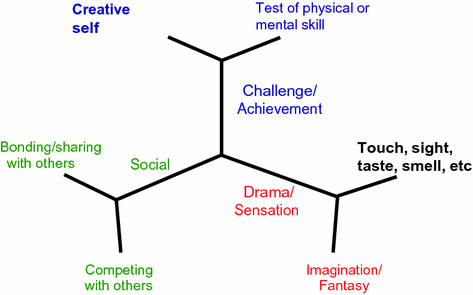
\includegraphics[width=0.9\linewidth]{figure/Analysis/provModelExp.png}
    	\caption{Provisional Model Of Consumer Experience\cite{Hull2018}}
    	\label{fig:provisionalModelOfConsumerExperience}
\end{figure}

\subsection{Designing for children}
When considering Zoo's population of visitors, a vast majority of the visitors are children of different ages(insert data from zoo when we get it here). Therefore, it is important to research and understand how to design for children as in comparison to adults. 
When designing for children, cognitive and physical development is an important matter to be considered\cite{kidsDesign}. Furthermore, the role of the family is also an important aspect when it comes to how the children perceive the digital experience\cite{kidsDesign}.

\subsection{Design principles}
When discussing design principles with the focus on children, a list of compiled principles have been made by the children's design guide\cite{kidsDesign}, which consists of a team of 70+ 'heroes' who come from different backgrounds such as designers, psychologist and neuroscientists. The ten principles can be seen in the list below:

\begin{enumerate}\label{princelist}
    \item \textbf{Everyone can play} I need a product that does not discriminate against characteristics such as gender, age, ability, language, ethnicity, and socio-economic status.
    \item \textbf{Give me control and offer support} Give me the tools I need to adapt to your product or service. Consider where I am in my development to both inspire me and nurture my growth.
    \item \textbf{I have purpose so make my influence matter} Help me understand my place and value in the world.
    \item \textbf{Offer me something safe} Ensure you provide me with a model for healthy behaviour, and do not forget that my data should be handled with utmost respect and care.
    \item \textbf{Create space for play (including a choice to chill)} When using your product or service, consider different moods, view and contexts of play.
    \item \textbf{Encourage me to be active and play with others} Provide me with experiences to help build relationships and social skills with my peers and community. 
    \item \textbf{Give me room to explore and experiment} I need to experiment, take risks and learn from my mistakes.
    \item \textbf{Use communication I can relate to} Consider all forms of communication, and make it accessible for all.
    \item \textbf{Make it flexible for me} Consider my open and fixed types of play or learning in your design.
    \item \textbf{You don’t know me, so make sure you include me} Spend time with me and my friends, we might have good ideas that can help you.
\end{enumerate}

To summarize the above principles, when designing for children it is important to focus on certain aspects of the design process. A focus which can be seen multiple times, is that when designing for children, it is important to provide space for the children to explore the product or the service on their own terms. Children have a tendency to use the product in each their own way, which can open to new ways of improving the product. Furthermore, it is important that communication, as well as the design, matches the children's level depending on the age group. 

It is also important to take safety into consideration when designing for children. The safety of a product is paramount, so when children interact with it, they, as well as the parents, can feel safe while doing so. The children need a safe environment while interacting, to efficiently grow, develop and mature\cite{safetyKids}.

While designing for children it is also important to incorporate the adults in one way or another. As Walt Disney said: "You are dead if you only aim for kids. Adults are grown up kids"\cite{safetyKids}. This means that if something is made ONLY for children, it is more likely to produce negative results.









%\section{The seven stages of action} % Simon
 %   The seven stages are awesomegaysauce. 

\subsection{Visual attention}\label{sec:visualAttention}

In "What attributes guide the deployment of visual attention and how do they do it?" Jeremy. M Wolfe explores which attributes guide visual attention\cite{Wolfe2004}.

For this an example image is shown:
\begin{figure}[H]
    	\centering
    	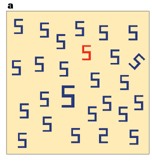
\includegraphics[width=0.4\linewidth]{figure/Analysis/natureFig1.png}
    	\caption{The red, the tilted or the big 5 are easy to find, the 2 not so much\cite{Wolfe2004}.}
    	\label{fig:hard2find}
    \end{figure}

Based on several features like the ones in the picture, tests were conducted to rank the time and efficiency with which they were isolated. The study resulted in a table of attributes that could guide attention

% Please add the following required packages to your document preamble:
% \usepackage[table,xcdraw]{xcolor}
% If you use beamer only pass "xcolor=table" option, i.e. \documentclass[xcolor=table]{beamer}
% \usepackage[normalem]{ulem}
% \useunder{\uline}{\ul}{}
\begin{table}[H]
\begin{tabular}{lllll}
\multicolumn{5}{l}{\textbf{Attributes that might guide the deployment of attention}}                                                                                                                                                                                                                                                                                                                                                                    \\
\rowcolor[HTML]{EFEFEF} 
\begin{tabular}[c]{@{}l@{}}Undoubted \\ attributes*\end{tabular}                            & \begin{tabular}[c]{@{}l@{}}Probable \\ attributes‡\end{tabular}        & \begin{tabular}[c]{@{}l@{}}Possible \\ attributes§\end{tabular}            & \begin{tabular}[c]{@{}l@{}}Doubtful \\ cases||\end{tabular}                                      & \begin{tabular}[c]{@{}l@{}}Probable \\ non-attributes¶\end{tabular}                              \\
Colour                                                                                      & \begin{tabular}[c]{@{}l@{}}Luminance \\ onset (flicker)\end{tabular}   & \begin{tabular}[c]{@{}l@{}}Lighting \\ direction \\ (shading)\end{tabular} & Novelty                                                                                          & Intersection                                                                                     \\
Motion                                                                                      & \begin{tabular}[c]{@{}l@{}}Luminance \\ polarity\end{tabular}          & \begin{tabular}[c]{@{}l@{}}Glossiness \\ (luster)\end{tabular}             & \begin{tabular}[c]{@{}l@{}}Letter identity \\ (over-learned \\ sets, \\ in general)\end{tabular} & \begin{tabular}[c]{@{}l@{}}Optic \\ flow\end{tabular}                                            \\
Orientation                                                                                 & \begin{tabular}[c]{@{}l@{}}Vernier \\ offset\end{tabular}              & Expansion                                                                  & \begin{tabular}[c]{@{}l@{}}Alphanumeric \\ category\end{tabular}                                 & \begin{tabular}[c]{@{}l@{}}Colour \\ change\end{tabular}                                         \\
\begin{tabular}[c]{@{}l@{}}Size (including \\ length and spatial \\ frequency)\end{tabular} & \begin{tabular}[c]{@{}l@{}}Stereoscopic \\ depth and tilt\end{tabular} & Number                                                                     &                                                                                                  & \begin{tabular}[c]{@{}l@{}}Three-\\ dimensional \\ volumes \\ (such as \\ geons)\end{tabular}    \\
                                                                                            & \begin{tabular}[c]{@{}l@{}}Pictorial \\ depth cues\end{tabular}        & \begin{tabular}[c]{@{}l@{}}Aspect \\ ratio\end{tabular}                    &                                                                                                  & \begin{tabular}[c]{@{}l@{}}Faces (Familar, \\ upright, angry \\ and so on)\end{tabular}          \\
                                                                                            & Shape                                                                  &                                                                            &                                                                                                  & Your name                                                                                        \\
                                                                                            & \begin{tabular}[c]{@{}l@{}}Line \\ termination\end{tabular}            &                                                                            &                                                                                                  & \begin{tabular}[c]{@{}l@{}}Semantic category \\ (for example, \\ 'animal', 'scary')\end{tabular} \\
                                                                                            & Closure                                                                &                                                                            &                                                                                                  &                                                                                                  \\
                                                                                            & \begin{tabular}[c]{@{}l@{}}Topological \\ status\end{tabular}          &                                                                            &                                                                                                  &                                                                                                  \\
                                                                                            & Curvature                                                              &                                                                            &                                                                                                  &                                                                                                 
\end{tabular}
\caption{"Attributes are grouped by the likelihood that they are, in fact, sources of guidance of attention. References are representative but not exhaustive. *‘Undoubted’ meaning
that they are supported by many studies with converging methods. ‡Less confidence owing to limited data, dissenting opinions or the possiblity of alternative
explanations. §Still less confidence. ||Unconvincing, but still possible. ¶Suggested guiding features where the balance of evidence argues against inclusion on the list"}
\label{table:attributesAttention}
\end{table}
\todo{This table caption is currently an exact copy\/paste of the article. How do we handle this?}

Considerations to include, if possible, all undoubted attributes as well as some probable attributes that guides attention should be made in the creation and installation of a display. All of these features are put into effect if they are different relative to their environment. For example if a display were of different luminance to it surroundings, it would potentially attract attention.


\subsection{Gamification}\todo{Det her kommer ud af ingenting lige nu, find ud af hvor vi bruger det.}
    The definition of gamification in this report is adhering to, is defined by Deterdin et al. as being: \begin{quote}
        \textit{"the use of game design elements in non-game contexts"}\cite{gamification}.
    \end{quote}
    Deterin et al. tries to define gamification due to the popularity the word has gained in both the industry and scientific space\cite{gamification}\todo{Hvad er formålet med denne sætning?}. According to another paper by Karl Kapp\cite{gamificationMyths}, there are four myths about the umbrella term \textit{gamification}\cite{gamificationMyths}. Of the four, two are the most relevant for this paper \todo{gennemgå afsnittet og konstater at alle "papers" mener artikler, og ikke vores raport}. The first myth, is that gamified interactions and games are the same, which is not the case\cite{gamificationMyths}. Games have a set end and beginning, while interaction based gamification don't necessarily have such beginning and ending\cite{gamificationMyths}. In games, the player usually has some expectation of a goal or win condition, while the same can't necessarily be said for a gamified interaction\cite{gamificationMyths}. The other myth is that gamification is all about points and achievements and rewards, and while these can play apart of a gamified experience, most games have much more than this\cite{gamificationMyths}. According to the paper, most games also have elements of story, challenge, continual feedback and a high level of interactivity, something that a gamified interaction doesn't have\cite{gamificationMyths}.\\
    
    An example of gamification is Khan Academy\footnote{Khan Academy: \url{https://www.khanacademy.org/}}. The website is used for learning various subjects, like mathematics, electrical engineering or physics, and tries to emphasize learning using a point system, streak counter for right answers and progress tracking per subject basis\cite{khanacademyGamfication}. This is a very rudimentary implementation of gamification, but it serves it's purpose of motivating a user to learn\cite{khanacademyGamfication}.

